\documentclass{uofsthesis-cs}

\usepackage{graphicx}
\usepackage{multirow}
\usepackage{amsmath}
\usepackage{algorithm2e}
\usepackage{listings}
\usepackage{float}
\usepackage{url}
\usepackage{hyperref}
\usepackage[T1]{fontenc}
\usepackage{enumitem}
\usepackage{booktabs}
\usepackage{nameref}
\usepackage{caption}
\usepackage{graphicx}
\newcommand{\superscript}[1]{\ensuremath{^{\textrm{#1}}}}
\newcommand{\subscript}[1]{\ensuremath{_{\textrm{#1}}}}
\renewcommand{\labelitemii}{$\star$}
\newcommand{\tabitem}{~~\llap{\textbullet}~~}
\newcommand{\specialcell}[2][c]{%
  \begin{tabular}[#1]{@{}c@{}}#2\end{tabular}}
\newcommand{\source}[1]{\caption*{ {#1}} }

% Documentation for the uofsthesis-cs class is given in uofsthesis-cs.dvi
% 
% It is recommended that you read the CGSR thesis preparation
% guidelines before proceeding.
% They can be found at http://www.usask.ca/cgsr/thesis/index.htm

%%%%%%%%%%%%%%%%%%%%%%%%%%%%%%%%%%%%%%%%%%%%%%%%%%%%%%%%%%%%%%%%%%%%%%%%%%%%%%
% FRONTMATTER - In this section, specify information to be used to
% typeset the thesis frontmatter.
%%%%%%%%%%%%%%%%%%%%%%%%%%%%%%%%%%%%%%%%%%%%%%%%%%%%%%%%%%%%%%%%%%%%%%%%%%%%%%

% THESIS TITLE
% Specify the title. Set the capitalization how you want it.
\title{Graphy: Exploring the Potential of the Contacts Application}

% AUTHOR'S NAME
% Your name goes here.
\author{Nam Hoang}

% DEGREE SOUGHT.  
% Use \MSc or \PhD here
\degree{\MSc}         

% EXPECTED CONVOCATION DATE
% Should be month/year, e.g. July 2004
\convocationdate{April/2016}


% NAME OF ACADEMIC UNIT
%
% The following two commands allow you to specify the academic unit you belong to.
% This will appear on the title page as
% ``<academic unit> of <department>''.
% So if you are in the division of biomedical engineering you would need to do:
% \department{Biomedical Engineering}
% \academicunit{Division}
%
% The default is ``Department of Computer Science'' if these commands
% are not given.
%
% If you are in a discipline other than Computer Science, uncomment the following line and
% specify your discipline/department.  Default is 'Computer Science'.
% \department{If not Computer Science, put the name of your department here}

% If you are not in a department, but say, a division, uncomment the following line.
% \academicunit{Put the type of academic unit you belong to here, e.g. Division, College}


% PERMISSION TO USE ADDRESS
%
% If you are not in Compuer Science you will want to change the
% address on the Permission to Use page.  This is done using the
% \ptuaddress{}.  Example:
%
% \ptuaddress{Head of the Department of Computer Science\\
% 176 Thorvaldson Building\\
% 110 Science Place\\
% University of Saskatchewan\\
% Saskatoon, Saskatchewan\\
% Canada\\
% S7N 5C9
% }

% ABSTRACT
\abstract{The number of mobile devices is growing very fast. Smart phones and tablets are, step by step, replacing desktops and laptops as the primary method of computing in daily life. Along with the rapid evolution of mobile devices, the applications on them are undergoing fast transformation. We can see many improvements in traditional applications (messaging, calling, etc.) like multimedia text messages, video calls, voice over IP and so forth. However, the Contacts application has not changed much while it has many potentials. In this thesis, we propose a new model which improves the Contacts application by introducing three novel capabilities: searching for contacts by their miscellaneous information, retaining knowledge of contacts via a tags system, and establishing a \textit{Personal Social Network} which consists of the relationships between the contacts. By introducing these capabilities, the model helps its users to accomplish new tasks which are not currently handled by modern Contacts applications. Furthermore, the model is implemented and become a fully functional prototype on iOS and Android. The prototype is then evaluated in a user study and a system performance test. The studies yield positive results which indicate that the three new capabilities are valuable and should be included in today's Contacts applications.}

% In this thesis, we explore the potentials of providing custom information, retaining historical context data in the Contacts application and connecting the contacts together based on their relationships. We implement a prototype of the new Contacts application which utilizes these three aspects then test it among a group of users. Our results are expected to indicate that custom information, historical context data and contact relationships are three important parts which should be included in today's Contacts applications.

% According to the 2014 annual report from Cisco \cite{cisco_report}, there were 406 million new smart phones and 92 million new tablets activated in 2013. Not only are smart devices increasing in popularity but they are becoming more and more powerful. The latest A8X chip which Apple uses for the iPad Air 2 contains 3 billion transistors and has 40\% more CPU performance and 2.5 times the graphics performance of its predecessor - the Apple A7 which had been released just a year before.

% THESIS ACKNOWLEDGEMENTS -- This can be free-form.
%\acknowledgements{
%I would like to express my gratitude to my supervisor, Dr. Ralph Deters, for his guidance, support and advice during the study.

%Furthermore, I am thankful to my committee members for their encouragement, valuable comments and suggestions.

%Finally, I wish to express my love and gratitude to my beloved family for their profound understanding and boundless love throughout the duration of my study.
%}


% THESIS DEDICATION -- Also free-form.  If you don't want a dedication, comment out the following
% line.
%\dedication{This is the thesis dedication (optional)}

% LIST OF ABBREVIATIONS - Sample  
% If you don't want a list of abbreviations, comment the following 4 lines.
%\loa{\abbrev{SCUBA}{Self Contained Underwater Breathing Apparatus}
%\abbrev{LOF}{List of Figures}
%\abbrev{LOT}{List of Tables}
%}

%%%%%%%%%%%%%%%%%%%%%%%%%%%%%%%%%%%%%%%%%%%%%%%%%%%%%%%%%%%%%%%%
% END OF FRONTMATTER SECTION
%%%%%%%%%%%%%%%%%%%%%%%%%%%%%%%%%%%%%%%%%%%%%%%%%%%%%%%%%%%%%%%%

\begin{document}

% Typeset the title page
\maketitle

% Typeset the frontmatter.  
\frontmatter

%%%%%%%%%%%%%%%%%%%%%%%%%%%%%%%%%%%%%%%%%%%%%%%%%%%%%%%%%%%%%%%%
% FIRST CHAPTER OF THESIS BEGINS HERE
%%%%%%%%%%%%%%%%%%%%%%%%%%%%%%%%%%%%%%%%%%%%%%%%%%%%%%%%%%%%%%%%

\input chapter1.tex
\input chapter2.tex
\input chapter3.tex
\input chapter4.tex
\input chapter5.tex
\input chapter6.tex

% Since thesis chapters are very long and there are a lot of them, it is recommended
% that you put each chapter in a separate .tex file and \input each one of them
% in order.  For example:
%
% \input chap1.tex
% \input chap2.tex
% ...
%
% The \input command inserts contents of the specified file at the point of the command.

%%%%%%%%%%%%%%%%%%%%%%%%%%%%%%%%%%%%%%%%%%%%%%%%%%%%%%%%%%%%%%%
% SUBSEQUENT CHAPTERS (or \input's)  GO HERE
%%%%%%%%%%%%%%%%%%%%%%%%%%%%%%%%%%%%%%%%%%%%%%%%%%%%%%%%%%%%%%%






%%%%%%%%%%%%%%%%%%%%%%%%%%%%%%%%%%%%%%%%%%%%%%%%%%%%%%%%%%%%%%%%
% The Bibliograpy should go here. BEFORE appendices!
%%%%%%%%%%%%%%%%%%%%%%%%%%%%%%%%%%%%%%%%%%%%%%%%%%%%%%%%%%%%%%%%


% Typeset the Bibliography.  The bibliography style used is "plain".
% Optionally, you can specify the bibliography style to use:
% \uofsbibliography[stylename]{yourbibfile}

\uofsbibliography{thesis_ref}

% If you are not using bibtex, comment the line above and uncomment
% the line below.  
%Follow the line below with a thebibliography environmentand bibitems.  
% Note: use of bibtex is usually the preferred method.

%\uofsbibliographynobibtex


%%%%%%%%%%%%%%%%%%%%%%%%%%%%%%%%%%%%%%%%%%%%%%%%%%%%%%%%%%%%%%%%%%%%%%%%%
% APPENDICES
%
% Any chapters appearing after the \appendix command get numbered with
% capital letters starting with appendix 'A'.
% New chapters from here on will be called 'Appendix A', 'Appendix B'
% as opposed to 'Chapter 1', 'Chapter 2', etc.
%%%%%%%%%%%%%%%%%%%%%%%%%%%%%%%%%%%%%%%%%%%%%%%%%%%%%%%%%%%%%%%%%%%%%%%%%%

% Activate thesis appendix mode.
\uofsappendix

\chapter{User Study Results}

% Table generated by Excel2LaTeX from sheet 'Sheet2'
\begin{table}[htbp]
  \centering
    \begin{tabular}{rrrrr}
    \toprule
    Index & Timestamp & All Searches & Traditional Searches & Traditional Searches Percentage \\
    \midrule
    1     & 11/4/15 & 31    & 19    & 0.6129 \\
    2     & 11/6/15 & 43    & 11    & 0.2558 \\
    3     & 11/6/15 & 26    & 14    & 0.5385 \\
    4     & 11/7/15 & 36    & 14    & 0.3889 \\
    5     & 11/10/15 & 73    & 6     & 0.0822 \\
    6     & 11/10/15 & 14    & 1     & 0.0714 \\
    7     & 11/11/15 & 12    & 0     & 0 \\
    8     & 11/17/15 & 36    & 18    & 0.5 \\
    9     & 11/18/15 & 36    & 15    & 0.4167 \\
    10    & 11/18/15 & 17    & 5     & 0.2941 \\
    11    & 11/19/15 & 30    & 12    & 0.4 \\
    12    & 11/20/15 & 20    & 7     & 0.35 \\
    13    & 11/20/15 & 16    & 4     & 0.25 \\
    14    & 11/21/15 & 29    & 9     & 0.3103 \\
    15    & 11/22/15 & 23    & 4     & 0.1739 \\
    16    & 11/23/15 & 42    & 11    & 0.2619 \\
    17    & 11/24/15 & 12    & 0     & 0 \\
    18    & 11/26/15 & 56    & 9     & 0.1607 \\
    19    & 11/28/15 & 59    & 5     & 0.0847 \\
    20    & 11/30/15 & 42    & 12    & 0.2857 \\
    21    & 11/30/15 & 20    & 6     & 0.3 \\
          &       &       &       &  \\
    Average &       & 32.0476 & 8.6667 & 0.2732 \\
    \bottomrule
    \end{tabular}%
  \label{tab:addlabel}%
\end{table}%

% Table generated by Excel2LaTeX from sheet 'Sheet3'
\begin{table}[htbp]
  \centering
    \begin{tabular}{rrrrr}
    \toprule
    Index & Tag Searches & \specialcell[t]{Tag Searches\\Percentage} & Relationship Searches & \specialcell[t]{Relationship Searches\\Percentage} \\
    \midrule
    1     & 12    & 0.3871 & 0     & 0 \\
    2     & 27    & 0.6279 & 5     & 0.1163 \\
    3     & 10    & 0.3846 & 2     & 0.0769 \\
    4     & 13    & 0.3611 & 9     & 0.25 \\
    5     & 57    & 0.7808 & 10    & 0.137 \\
    6     & 13    & 0.9286 & 0     & 0 \\
    7     & 9     & 0.75  & 3     & 0.25 \\
    8     & 17    & 0.4722 & 1     & 0.0278 \\
    9     & 13    & 0.3611 & 8     & 0.2222 \\
    10    & 10    & 0.5882 & 2     & 0.1176 \\
    11    & 12    & 0.4   & 6     & 0.2 \\
    12    & 12    & 0.6   & 1     & 0.05 \\
    13    & 9     & 0.5625 & 3     & 0.1875 \\
    14    & 12    & 0.4138 & 8     & 0.2759 \\
    15    & 15    & 0.6522 & 4     & 0.1739 \\
    16    & 25    & 0.5952 & 6     & 0.1429 \\
    17    & 10    & 0.8333 & 2     & 0.1667 \\
    18    & 40    & 0.7143 & 7     & 0.125 \\
    19    & 46    & 0.7797 & 8     & 0.1356 \\
    20    & 21    & 0.5   & 9     & 0.2143 \\
    21    & 10    & 0.5   & 4     & 0.2 \\
          &       &       &       &  \\
    Average & 18.7143 & 0.5806 & 4.6667 & 0.1462 \\
    \bottomrule
    \end{tabular}%
  \label{tab:addlabel}%
\end{table}%

% Table generated by Excel2LaTeX from sheet 'Sheet4'
\begin{table}[htbp]
  \centering
    \begin{tabular}{rrrrrr}
    \toprule
    Index & \specialcell[t]{Tag Used\\in Seaches} & Tags per search & \specialcell[t]{Relationship Used\\in Searches} & \specialcell[t]{Relationships\\per search} & \specialcell[t]{Relationship\\Navigations} \\
    \midrule
    1     & 13    & 1.0833 & 0     & 0     & 17 \\
    2     & 30    & 1.1111 & 5     & 1     & 62 \\
    3     & 10    & 1     & 2     & 1     & 31 \\
    4     & 13    & 1     & 9     & 1     & 3 \\
    5     & 57    & 1     & 10    & 1     & 15 \\
    6     & 13    & 1     & 0     & 0     & 3 \\
    7     & 9     & 1     & 3     & 1     & 16 \\
    8     & 17    & 1     & 1     & 1     & 21 \\
    9     & 13    & 1     & 8     & 1     & 5 \\
    10    & 10    & 1     & 2     & 1     & 16 \\
    11    & 12    & 1     & 6     & 1     & 14 \\
    12    & 12    & 1     & 1     & 1     & 15 \\
    13    & 9     & 1     & 3     & 1     & 21 \\
    14    & 15    & 1.25  & 8     & 1     & 9 \\
    15    & 16    & 1.0667 & 4     & 1     & 32 \\
    16    & 27    & 1.08  & 6     & 1     & 53 \\
    17    & 10    & 1     & 2     & 1     & 11 \\
    18    & 40    & 1     & 7     & 1     & 21 \\
    19    & 46    & 1     & 8     & 1     & 15 \\
    20    & 21    & 1     & 9     & 1     & 5 \\
    21    & 11    & 1.1   & 4     & 1     & 14 \\
          &       &       &       &       &  \\
    Average & 19.2381 & 1.0329 & 4.6667 & 0.9048 & 19 \\
    \bottomrule
    \end{tabular}%
  \label{tab:addlabel}%
\end{table}%

% Table generated by Excel2LaTeX from sheet 'Sheet5'
\begin{table}[htbp]
  \centering
    \begin{tabular}{rrrrrr}
    \toprule
    Index & \specialcell[t]{Active Contacts\\Total} & Tags Total & Tags Average & Relationships Total & Relationships Average \\
    \midrule
    1     & 46    & 180   & 3.913 & 94    & 2.0435 \\
    2     & 72    & 241   & 3.3472 & 146   & 2.0278 \\
    3     & 55    & 127   & 2.3091 & 67    & 1.2182 \\
    4     & 16    & 27    & 1.6875 & 30    & 1.875 \\
    5     & 50    & 101   & 2.02  & 87    & 1.74 \\
    6     & 9     & 22    & 2.4444 & 7     & 0.7778 \\
    7     & 8     & 29    & 3.625 & 12    & 1.5 \\
    8     & 49    & 165   & 3.3673 & 86    & 1.7551 \\
    9     & 20    & 48    & 2.4   & 39    & 1.95 \\
    10    & 18    & 69    & 3.8333 & 34    & 1.8889 \\
    11    & 32    & 68    & 2.125 & 45    & 1.4063 \\
    12    & 29    & 67    & 2.3103 & 33    & 1.1379 \\
    13    & 23    & 60    & 2.6087 & 29    & 1.2609 \\
    14    & 24    & 47    & 1.9583 & 38    & 1.5833 \\
    15    & 30    & 102   & 3.4   & 58    & 1.9333 \\
    16    & 63    & 207   & 3.2857 & 128   & 2.0317 \\
    17    & 8     & 26    & 3.25  & 10    & 1.25 \\
    18    & 52    & 111   & 2.1346 & 80    & 1.5385 \\
    19    & 41    & 85    & 2.0732 & 71    & 1.7317 \\
    20    & 22    & 41    & 1.8636 & 41    & 1.8636 \\
    21    & 17    & 56    & 3.2941 & 31    & 1.8235 \\
          &       &       &       &       &  \\
    Average & 32.5714 & 89.4762 & 2.7262 & 55.5238 & 1.6351 \\
    \bottomrule
    \end{tabular}%
  \label{tab:addlabel}%
\end{table}%

% Table generated by Excel2LaTeX from sheet 'Sheet6'
\begin{table}[htbp]
  \centering
    \begin{tabular}{rrrrr}
    \toprule
    Index & Tag Weight Average & Relationship Weight Average & \specialcell[t]{Tag Types\\Total} & \specialcell[t]{Relationship Types\\Total} \\
    \midrule
    1     & 0.3541 & 0.1842 & 114   & 23 \\
    2     & 0.3446 & 0.1823 & 106   & 36 \\
    3     & 0.2913 & 0.1627 & 126   & 36 \\
    4     & 0.1686 & 0.2229 & 27    & 14 \\
    5     & 0.1811 & 0.1437 & 91    & 11 \\
    6     & 0.3075 & 0.0956 & 29    & 4 \\
    7     & 0.3047 & 0.1691 & 30    & 5 \\
    8     & 0.3365 & 0.1782 & 117   & 27 \\
    9     & 0.1943 & 0.2175 & 39    & 15 \\
    10    & 0.3177 & 0.1731 & 52    & 10 \\
    11    & 0.2186 & 0.1984 & 67    & 23 \\
    12    & 0.3006 & 0.1243 & 64    & 18 \\
    13    & 0.3002 & 0.1669 & 42    & 15 \\
    14    & 0.1947 & 0.21  & 39    & 17 \\
    15    & 0.3184 & 0.1736 & 56    & 16 \\
    16    & 0.317 & 0.1887 & 94    & 33 \\
    17    & 0.3057 & 0.1424 & 20    & 5 \\
    18    & 0.2215 & 0.1507 & 104   & 20 \\
    19    & 0.2083 & 0.1493 & 78    & 10 \\
    20    & 0.171 & 0.2078 & 39    & 13 \\
    21    & 0.2859 & 0.1829 & 45    & 10 \\
          &       &       &       &  \\
    Average & 0.2687 & 0.1726 & 65.6667 & 17.1905 \\
    \bottomrule
    \end{tabular}%
  \label{tab:addlabel}%
\end{table}%

\chapter{Database Schema}

\begin{figure}[!h]
\begin{center}
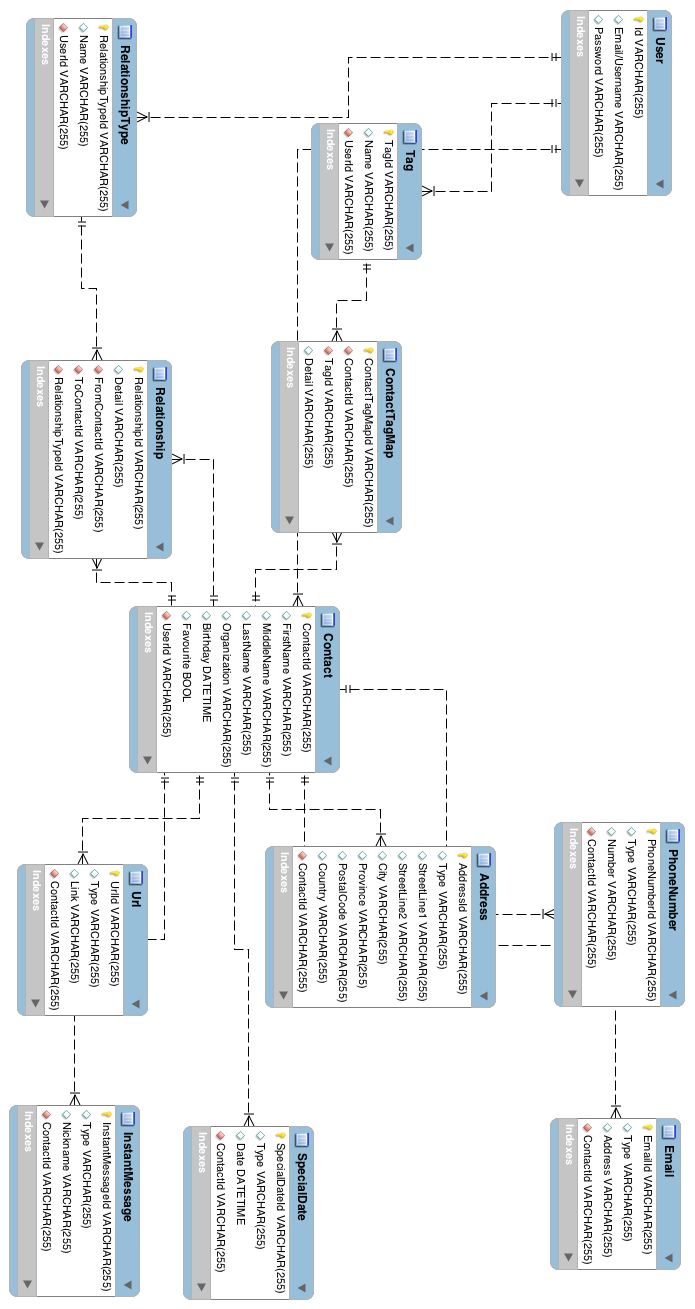
\includegraphics[scale=0.5]{pics/full_schema.png}
%\caption{Sync Queue Table}\label{fg:full_schema}
\end{center}
\end{figure}

\chapter{User Study Online Survey}

\begin{figure}[!h]
\begin{center}
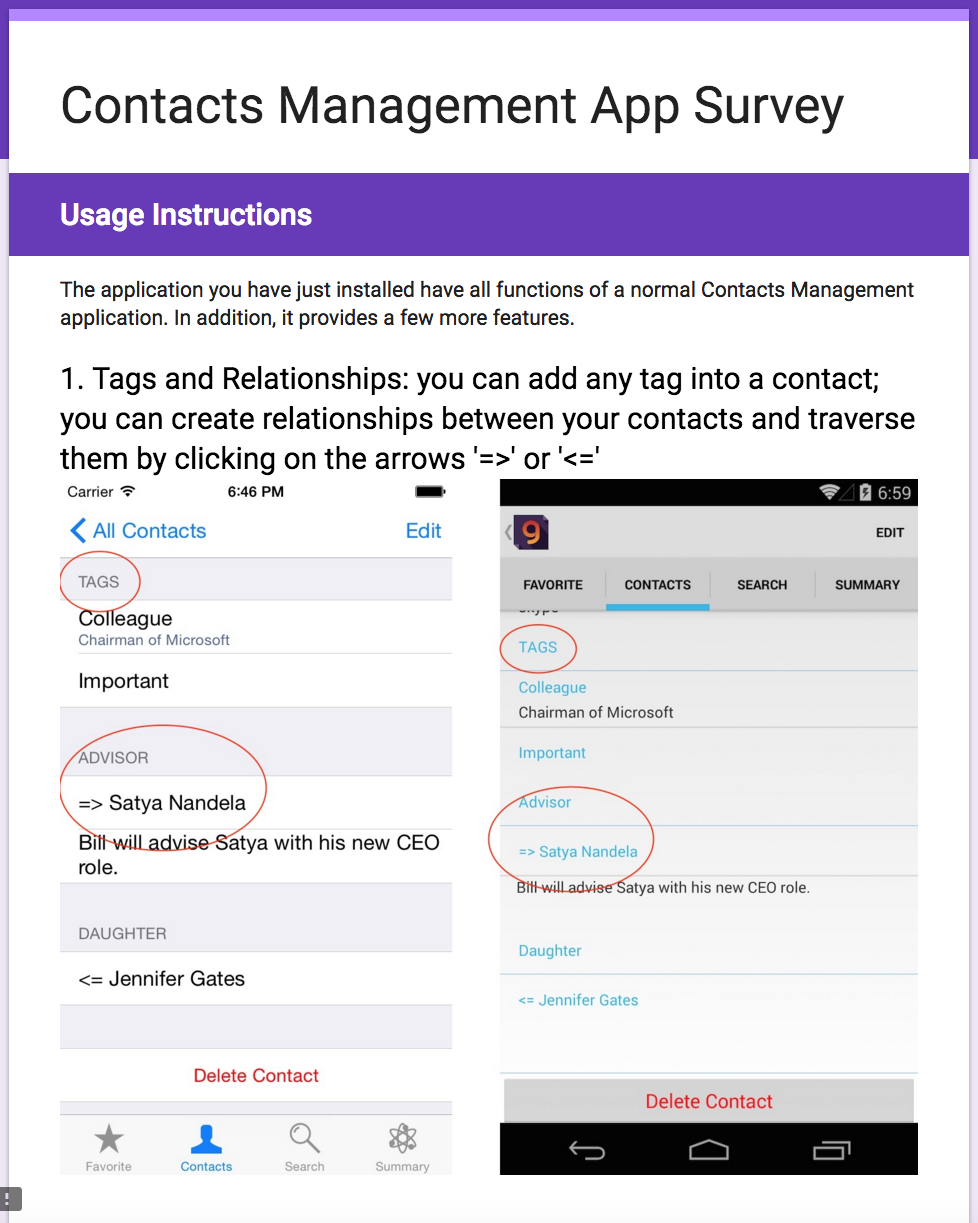
\includegraphics[scale=0.4]{pics/survey1.png}
\end{center}
\end{figure}

\begin{figure}[!h]
\begin{center}
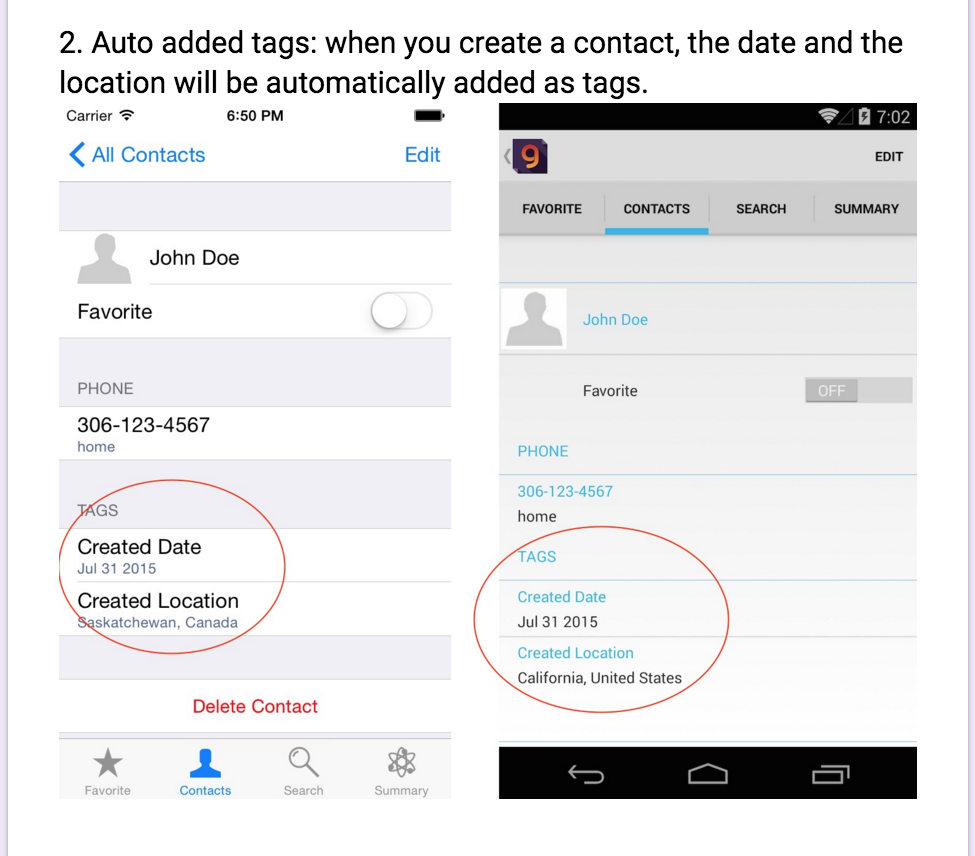
\includegraphics[scale=0.4]{pics/survey2.png}
\end{center}
\end{figure}

\begin{figure}[!h]
\begin{center}
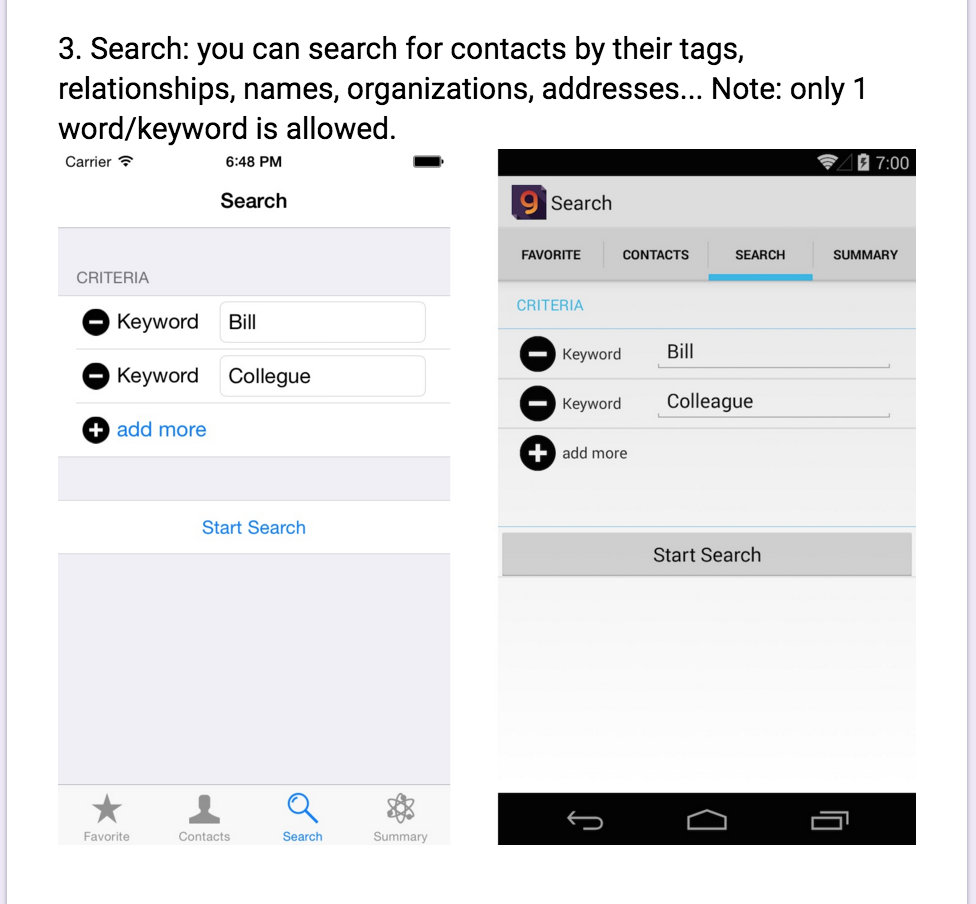
\includegraphics[scale=0.4]{pics/survey3.png}
\end{center}
\end{figure}

\begin{figure}[!h]
\begin{center}
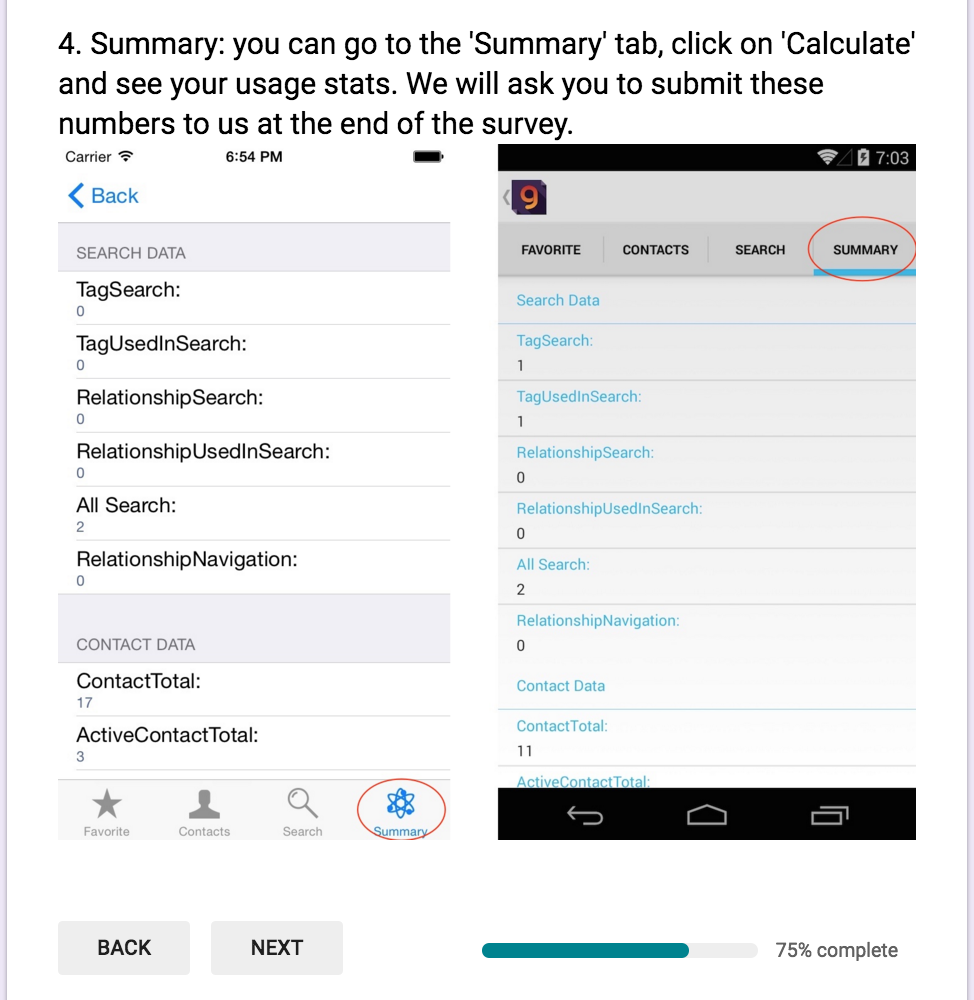
\includegraphics[scale=0.4]{pics/survey4.png}
\end{center}
\end{figure}

\begin{figure}[!h]
\begin{center}
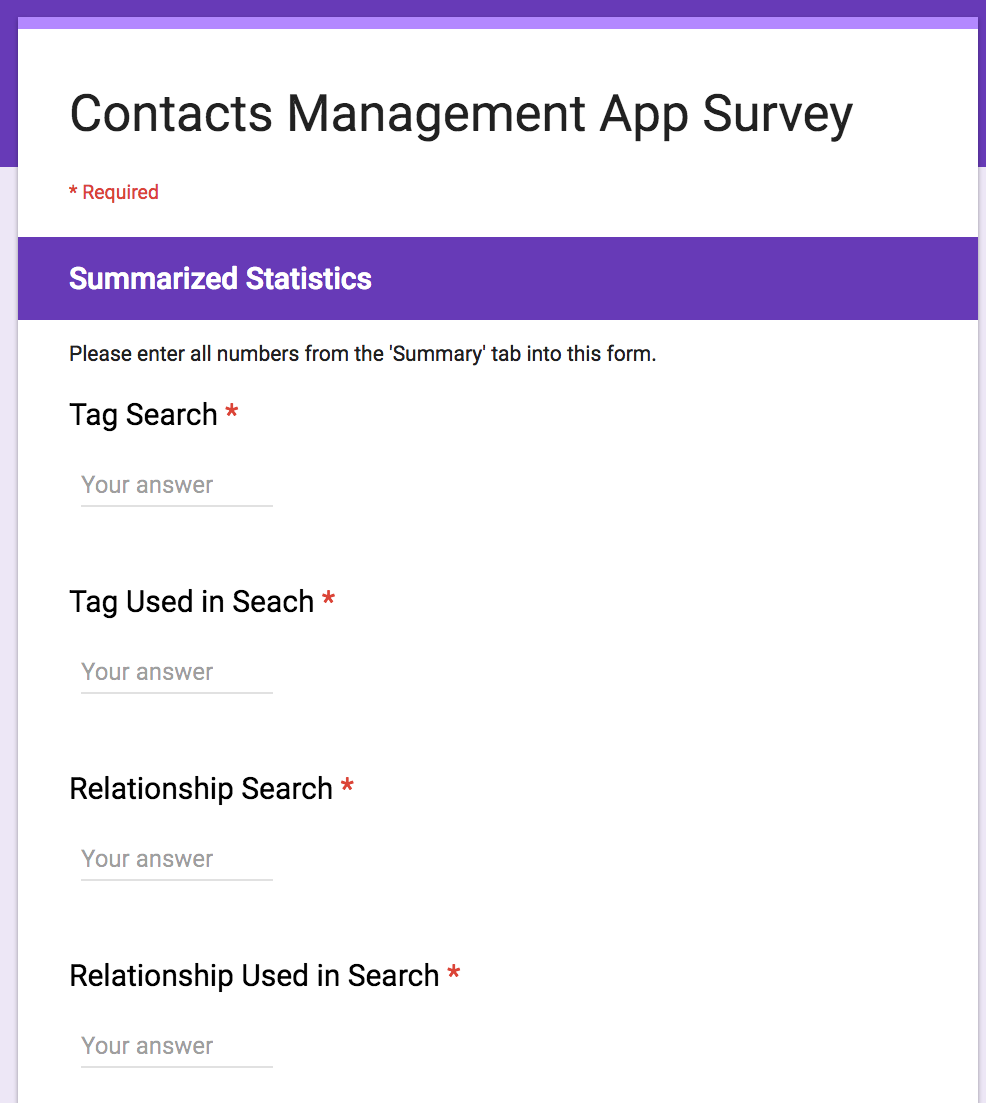
\includegraphics[scale=0.4]{pics/survey5.png}
\end{center}
\end{figure}

\begin{figure}[!h]
\begin{center}
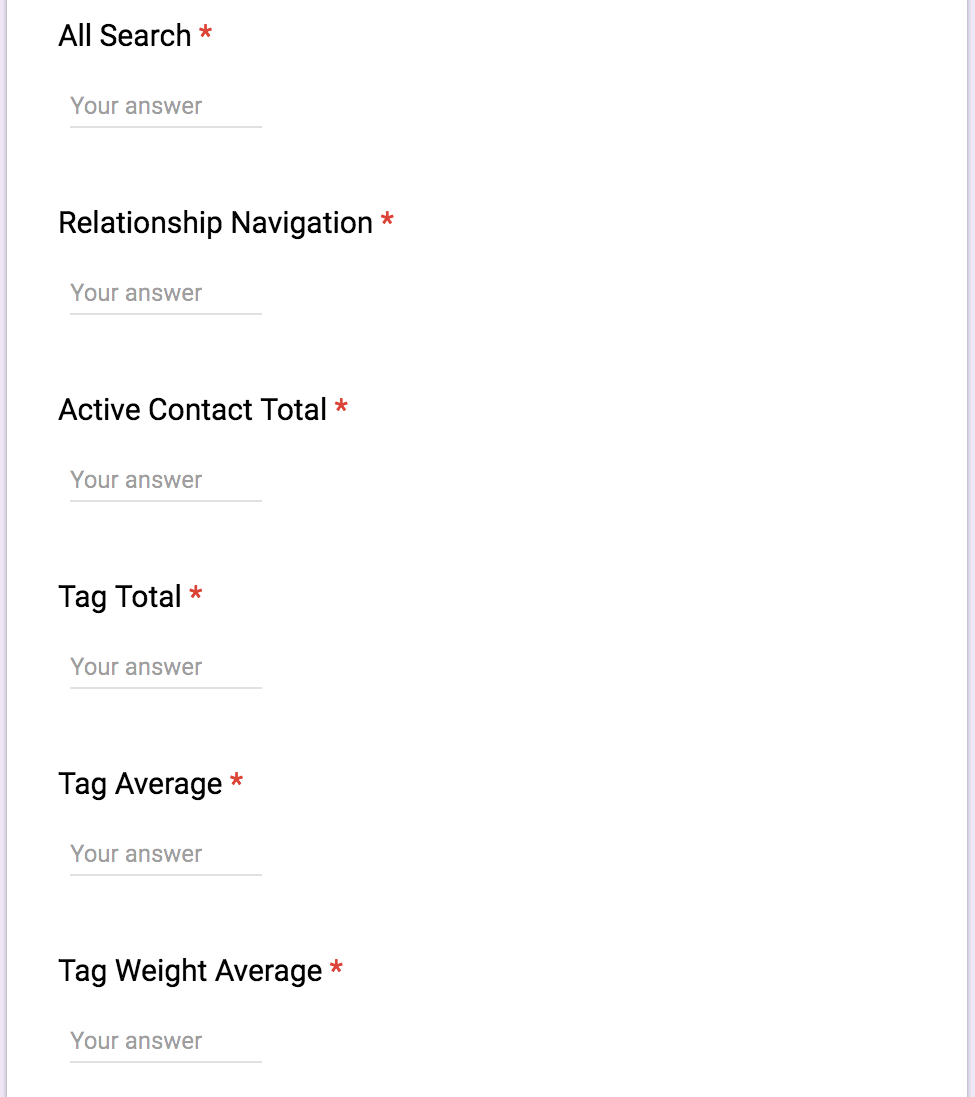
\includegraphics[scale=0.4]{pics/survey6.png}
\end{center}
\end{figure}

\begin{figure}[!h]
\begin{center}
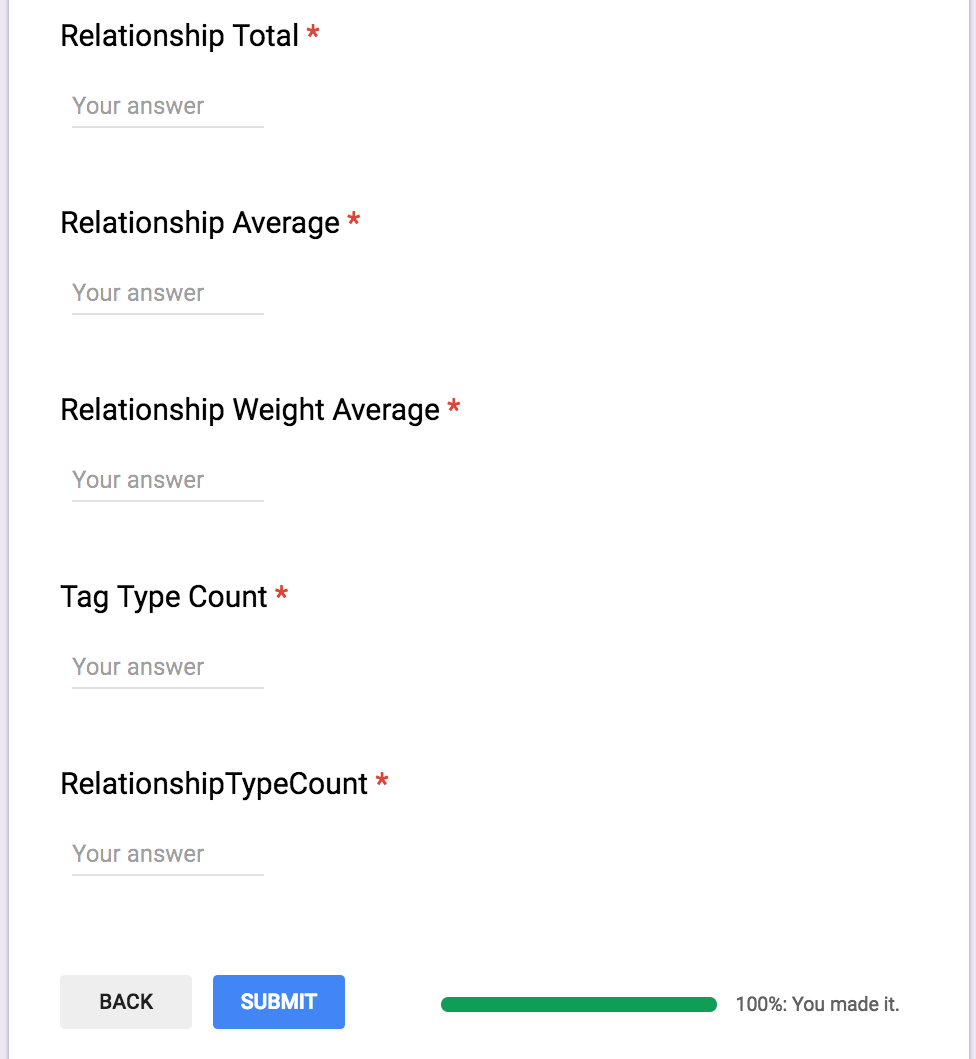
\includegraphics[scale=0.4]{pics/survey7.png}
\end{center}
\end{figure}

\end{document}
